\documentclass{tufte-handout}

\usepackage[french]{babel}
\usepackage[utf8]{inputenc}
\usepackage[T1]{fontenc}
\usepackage{amsmath, amsthm, amsfonts}
\usepackage{siunitx}
\usepackage{tikz}
\usepackage{hyperref}
%\usepackage[backend=biber, autocite=footnote]{biblatex}
\usepackage{xcolor}
\usepackage{caption}
\usepackage{booktabs}
\usepackage{mathtools}

\tikzset{>=latex}
\usetikzlibrary{calc,decorations.pathreplacing}
\sisetup{locale=FR, per-mode=symbol}

\newcommand{\abs}[1]{\left| #1 \right|}
%\renewcommand{\vec}[1]{\ensuremath{\overrightarrow{\boldsymbol{\mathrm{ #1 }}}}}
\newcommand{\rhat}{\vec{\hat{r}}}
\newcommand{\xhat}{\vec{i}}
\newcommand{\yhat}{\vec{j}}
\newcommand{\zhat}{\vec{k}}
\newcommand{\real}{\mathbb{R}}
\newcommand{\der}[2]{\frac{\mathrm{d}#1}{\mathrm{d}#2}}
\newcommand{\pder}[2]{\frac{\partial #1}{\partial #2}}
\newcommand{\dif}{\mathrm{d}}
\newcommand{\ddif}{\,\mathrm{d}}
\newcommand{\grad}{\vec{\nabla}}
\newcommand{\exemple}[1]{\begin{fullwidth}#1\end{fullwidth}}
\newcommand{\norm}[1]{\lVert #1 \rVert}
\newcommand{\vu}{\vec{u}}
\newcommand{\vv}{\vec{v}}
\newcommand{\vr}{\vec{r}}
\newcommand{\va}{\vec{a}}
\newcommand{\vF}{\vec{F}}
\newcommand{\vecxyz}[3]{#1 \xhat + #2 \yhat + #3 \zhat}
\newcommand{\vecxy}[2]{#1 \xhat + #2 \yhat}

\theoremstyle{definition}
\newtheorem*{defn}{Definition}



\title{Exemples sur l'équilibre statique}
\date{}

\begin{document}

\maketitle
\vspace{0.5cm}

\section{Le laveur de vitre}

Un laveur de vitre de \SI{70}{\kilogram} se tient à \SI{1.5}{\meter} de
l'extrémité d'une plateforme de \SI{10}{\kilogram} retenue par deux câbles
fixés à ses extrémités.  Si la longueur de la plateforme est de \SI{5}{\meter},
déterminer le module de la tension dans chacun des câbles.

On définit les variables suivantes
\begin{align*}
  m &= \SI{70}{\kilogram}  & \text{(masse du laveur)} \\
  M &= \SI{10}{\kilogram}  & \text{(masse de la plateforme)} \\ 
  d &= \SI{1.5}{\meter}  & \text{(distance entre le laveur et l'extrémité)} \\ 
  L &= \SI{5}{\meter}  & \text{(longueur de la plateforme)} \\ 
\end{align*}

Ce problème est une situation d'équilibre statique, il est donc possible de
définir l'axe de rotation n'importe où.  On choisit un axe de rotation qui
passe par le point d'application d'une des forces, soit la tension dans le
câble de gauche (la position de l'axe de rotation est indiquée par un point
rouge dans la figure ci-contre).  Le sens positif de rotation est le sens
antihoraire et l'axe des $y$ est orienté vers le haut.

\begin{marginfigure}
  \begin{center}
  \begin{tikzpicture}[scale=0.4]
    \draw[ultra thick] (-4, 0) -- (4, 0);
    \draw (-3.9, 0) -- (-3.9, 4);
    \draw (3.9, 0) -- (3.9, 4);
    \draw (2, 1) -- (2, 2.6)
          (1.5, 0) -- (2, 1)
          (2.5, 0) -- (2, 1)
          (2, 2.1) -- (1.3, 3)
          (2, 2.1) -- (2.7, 3);
    \draw (2, 3) circle (0.4);
    \draw[very thick, blue, ->] (-4.1, 0) -- node[left] {$\vec{T}_1$} (-4.1, 3);
    \draw[very thick, blue, ->] (4.1, 0) -- node[right] {$\vec{T}_2$} (4.1, 3);
    \draw[very thick, blue, ->] (0, 0) -- node[left] {$\vec{F}_{g1}$} (0, -3);
    \draw[very thick, blue, ->] (2, 0) -- node[right] {$\vec{F}_{g2}$} (2, -4);
    \fill[red] (-4, 0) circle (5pt);
    \draw[->] (7, 4) arc (0:270:1);
    \node at (6, 4) {$\boldsymbol{+}$};
    \draw[->] (-6, -2) -- (-6, 3) node[left] {$y$};
  \end{tikzpicture}
  \end{center}
\end{marginfigure}

La somme des forces en $y$ doit être nulle parce qu'il s'agit d'une situation
d'équilibre statique:
\begin{align}
  \label{eq:forces}
  \sum F_y &= T_1 + T_2 - mg - Mg = 0.
\end{align}
La somme des moments de force doit aussi être nulle:
\begin{align}
  \label{eq:moments}
  \sum \tau &= \tau_{T_1} + \tau_{T_2} + \tau_{m} + \tau_{M} \nonumber \\
            &= 0 + LT_2 - (L - d)mg - \frac{1}{2} L Mg = 0
\end{align}
Le facteur $\sin\theta$ n'apparaît pas parce que toutes les forces font un
angle de \SI{90}{\degree} avec le segment de droite reliant leur point
d'application à l'axe de rotation.  Pour expliquer le choix des signes, il faut
réaliser que les deux poids ont tendance à faire tourner la passerelle dans le
sens négatif alors que la tension de droite a tendance à la faire tourner dans
le sens positif.

De l'équation \ref{eq:moments} on peut isoler $T_2$:
\begin{align*}
  T_2 &= \frac{L - d}{L} mg + \frac{1}{2}Mg \\
      &= \SI{529.2}{\newton}
\end{align*}
\begin{equation*}
  \boxed{T_2 = \SI{529}{\newton}}
\end{equation*}

De l'équation \ref{eq:forces} on peut isoler $T_1$:
\begin{align*}
  T_1 &= -T_2 + mg + Mg \\
      &= \SI{254.8}{\newton}
\end{align*}
\begin{equation*}
  \boxed{T_1 = \SI{255}{\newton}}
\end{equation*}

La tension dans le câble le plus près du laveur de vitre est plus grande que
l'autre câble parce qu'il doit supporter une plus grande partie du poids du
laveur.


\section{La poutre}

Une poutre de \SI{20.0}{kg} mesurant \SI{4.00}{m} est retenue par un câble dont
la tension de rupture vaut \SI{1000}{N}. La poutre fait un angle de
\SI{30.0}{\degree} par rapport à l'horizontale. Le câble est perpendiculaire à
la poutre et est fixé à \SI{3.00}{m} du pivot.  Déterminer

\begin{enumerate}
  \item la charge maximale en kg que l'on peut suspendre à l'extrémité de la poutre
  \item les composantes horizontale et verticale de la force exercée par le
    pivot dans ce
cas.
\end{enumerate}


\begin{marginfigure}
  \begin{center}
  \begin{tikzpicture}[scale=0.5]
    \draw (0, -3) -- (0, 3);
    \draw[double] (4.5, 2.9) -- ++(120:4);
    \draw[double] (6.2, 3.3) -- ++(0, -3);
    \draw[shift={(0.2, 0)}, rotate=30, fill=black!20] (0, -0.3) rectangle (7, 0.3);
    \draw[fill=black!50] (0, -0.5) arc (-90:90:0.5);
    \fill[red] (0.25, 0) circle (5pt);
    \draw[rounded corners] (5.5, -1) rectangle node {$m$} (6.9, 0.3);
    \draw[very thick, blue, ->] (4.7, 3) -- node[left] {$\vec{T}_{\mathrm{max}}$} ++(120:3);
    \draw[very thick, blue, ->] (6.4, 3.1) -- node[right] {$\vec{F}_{gm}$} ++(0, -2);
    \draw[very thick, blue, ->, shift={(30:3.5)}] (0, 0) -- node[left] {$\vec{F}_{gM}$} (0, -3);
    \draw[very thick, blue, ->, shift={(0.4,0.4)}] (0, 0) -- ++(70:3) node[anchor=south east] {$\vec{F}_{p}$};
    \draw[->] (8, 6) arc (0:270:1);
    \node at (7, 6) {$\boldsymbol{+}$};
    \draw[->] (7, -4) -- (7, -3) node[left] {$y$};
    \draw[->] (7, -4) -- (8, -4) node[below] {$x$};  
  \end{tikzpicture}
  \end{center}
\end{marginfigure}

En plus des forces dessinées dans le schéma ci-contre, on définit les variables
suivantes
\begin{align*}
  m &  & \text{(masse suspendue)} \\
  M &= \SI{20}{\kilogram}  & \text{(masse de la poutre)} \\ 
  d &= \SI{3}{\meter}  & \text{(distance entre le pivot et le point d'attache
    du câble)} \\ 
  L &= \SI{4}{\meter}  & \text{(longueur de la poutre)} \\ 
  \theta &= \SI{30}{\degree}  & \text{(angle entre la poutre et l'horizontale)} \\ 
\end{align*}

Puisqu'on cherche la charge maximale, on peut supposer que le module de la
tension dans le câble est égal à la tension de rupture.  La direction de la
force exercée par le pivot sur la poutre est arbitraire dans la figure.

L'axe de rotation est perpendiculaire à la page et passe par le pivot (point
rouge dans la figure).  On utilise cet axe de rotation parce que le moment de
force pour la force exercée par le pivot sera nulle.  Puisqu'on ne connaît pas
l'orientation de cette force, il est préférable d'éviter d'avoir à écrire une
expression pour le moment de force correspondant.

En situation d'équilibre statique, le moment de force total est nul. Avant de
faire la somme, il faut déterminer les moments de force de chacune des quatre
forces dans le problème.

\paragraph{$\vF_p$:}
$\tau_p = 0$ car la force est appliquée au même endroit que l'axe de rotation.
Par conséquent, la distance entre le point d'application de la force et l'axe
de rotation est nulle.


\paragraph{$\vec{T}_\mathrm{max}$:}
L'angle entre le vecteur qui va de l'axe de rotation au point d'application de
la force, $\vec{r}_T$, et la tension dans le câble est de \SI{90}{\degree}.  Si
seule la tension agissait sur la poutre, elle décrirait une rotation dans le
sens positif.  Par conséquent, le moment de force est
\begin{marginfigure}
  \begin{center}
    \begin{tikzpicture}[scale=0.5]
      \draw[thick, ->] (0, 0) -- node[anchor=north west] {$\vec{r}_T$} ++(30:5);
      \draw[thick, ->] (30:5) -- node[anchor=south west] {$\vec{T}_\mathrm{max}$} ++(120:4);
      \draw[densely dashed] (30:5) -- ++(30:2);
      \fill[rotate=30] (5, 0) rectangle (5.3, 0.3);
      \fill[red] (0, 0) circle (4pt);
    \end{tikzpicture}
  \end{center}
\end{marginfigure}
\begin{align*}
  \tau_T &= r_T T_\mathrm{max} \sin \SI{90}{\degree} \\
         &= dT_\mathrm{max}.
\end{align*}


\paragraph{$\vec{F}_{gM}$:}
La force de gravité sur la poutre agit au centre de masse.  En supposant que la
poutre est uniforme, le centre de masse est situé au centre géométrique, soit à
une distance $L/2$ de l'axe de rotation.  L'angle entre le vecteur qui va de
l'axe de rotation au point d'application de la force, $\vec{r}_M$, et le poids
de la poutre est de $\theta + \SI{90}{\degree}$.  Si seul le poids de la
poutre agissait sur la poutre, elle décrirait une rotation dans le sens
négatif.  Par conséquent, le moment de force est
\begin{marginfigure}
  \begin{center}
    \begin{tikzpicture}[scale=0.5]
      \draw[thick, ->] (0, 0) -- node[anchor=south east] {$\vec{r}_M$} ++(30:4);
      \draw[thick, ->] (30:4) -- ++(0, -3) node[right] {$\vec{F}_{gM}$};
      \draw[densely dashed] (30:4) -- ++(30:3);
      \draw[densely dashed] (0, 0) -- (2, 0);
      \draw[densely dashed] (30:4) -- ++(2, 0);
      \draw (1, 0) arc (0:30:1);
      \draw ($(30:4) + (1, 0)$) arc (0:30:1);
      \node at (15:1.6) {$\theta$};
      \node at ($(30:4) + (15:1.6)$) {$\theta$};
      \fill[red] (0, 0) circle (4pt);
    \end{tikzpicture}
  \end{center}
\end{marginfigure}
\begin{align*}
  \tau_M &= -r_M Mg \sin (\theta + \SI{90}{\degree}) \\
         &= - \frac{L}{2} Mg \cos\theta
\end{align*}


\paragraph{$\vec{F}_{gm}$:}
Le poids de la masse suspendue agit sur la
poutre (via une corde de masse négligeable) à une distance $L$ de l'axe de
rotation.  Le reste du raisonnement pour trouver le moment de force est
identique à celui pour le poids de la poutre.  On obtient
\begin{align*}
  \tau_m &= - L mg \cos\theta
\end{align*}


Le moment de force total est donc
\begin{align*}
  \tau &= \tau_p + \tau_T + \tau_M + \tau_m \\
       &= dT_\mathrm{max} - \frac{L}{2} Mg \cos\theta - Lmg\cos\theta \\
       &= 0 & \text{car équilibre statique}
\end{align*}
De cette équation, on peut isoler $m$:
\begin{align*}
  m &= \frac{dT_\mathrm{max}}{Lg\cos\theta} - \frac{M}{2}
\end{align*}
\begin{equation*}
  \boxed{m = \SI{78.4}{\kilogram}}
\end{equation*}


Pour trouver les composantes de la force exercée par le pivot, on utilise le
fait que dans une situation d'équilibre statique, la somme des forces est aussi
nulle.
\begin{marginfigure}
  \begin{center}
    \begin{tikzpicture}[scale=0.5]
      \draw[thick, ->] (0, 0) -- node[above] {$\vec{r}_T$} ++(30:5);
      \draw[thick, ->] (30:5) -- node[left] {$\vec{T}_\mathrm{max}$} ++(120:4);
      \draw[densely dashed] (30:5) -- ++(30:2);
      \fill[rotate=30] (5, 0) rectangle (5.3, 0.3);
      \draw[densely dashed] (0, 0) -- (3, 0);
      \draw (1, 0) arc (0:30:1);
      \node at (15:1.6) {$\theta$};
      \draw[densely dashed] (30:5) -- ++(3, 0);
      \draw[densely dashed] (30:5) -- ++(0, 3);
      \draw ($(30:5) + (1, 0)$) arc (0:30:1);
      \node at ($(30:5) + (15:1.6)$) {$\theta$};
      \draw ($(30:5) + (0, 1)$) arc (90:120:1);
      \node at ($(30:5) + (105:1.6)$) {$\theta$};
      \fill[red] (0, 0) circle (4pt);
    \end{tikzpicture}
  \end{center}
\end{marginfigure}
\begin{align*}
  \sum F_x &= F_{px} - T_\mathrm{max} \sin\theta = 0 \\
  F_{px} &= T_\mathrm{max} \sin\theta
\end{align*}
\begin{equation*}
  \boxed{F_{px} = \SI{500}{\newton}}
\end{equation*}
\begin{align*}
  \sum F_y &= F_{py} + T_\mathrm{max} \cos\theta - Mg - mg = 0 \\
  F_{px} &= Mg + mg - T_\mathrm{max} \cos\theta
\end{align*}
\begin{equation*}
  \boxed{F_{py} = \SI{98.0}{\newton}}
\end{equation*}


\section{\textbf{Bonus!} Quelle est la masse de Darth Vader?}

Grâce à nos connaissances sur l'équilibre statique, nous sommes maintenant en
mesure de calculer la masse de Darth Vader. Nous utiliserons une séquence de
\textit{Star Wars IV: A New Hope} lors de laquelle Darth Vader soulève un
officier rebelle en lui demandant ``If this is a consular ship, where is the
ambassador?''

\begin{figure}
\begin{center}
  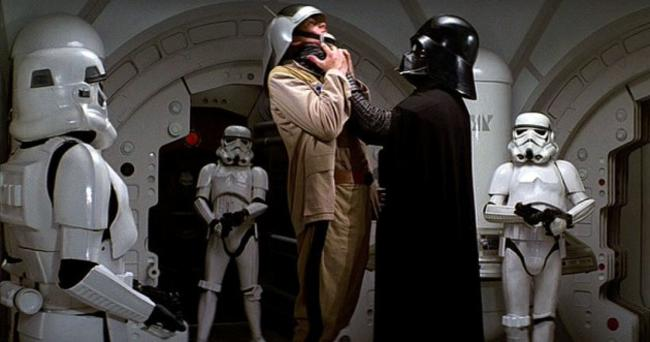
\includegraphics[scale=1]{vader_consular_ship.jpg}
\end{center}
\end{figure}

D'abord, nous pouvons représenter schématiquement la situation par la figure
ci-dessous.  Le bloc de gauche représente l'officier rebelle alors que le bloc
de droite représente Vader.  Nous supposons que la masse du bras de Vader est
négligeable par rapport aux masses de Vader et du rebelle.

Dans ce problème, il y a trois forces à considérer: le poids du rebelle, le
poids de Vader et la force normale exercée par le plancher sur les pieds de
Vader.  Étant donné qu'il soulève une masse, Vader sera porté à basculer vers
l'avant et la force normale du plancher agira donc sur la partie la plus
avancée de ses pieds, c'est-à-dire ses orteils.  Sur la photo, Vader semble se
tenir très droit, donc il est raisonnable d'estimer la position de ses
orteils à $l = \SI{10}{\centi\meter}$ devant son centre de masse.

\begin{marginfigure}
  \begin{center}
    \begin{tikzpicture}[scale=0.5]
      \draw (0, 1.5) rectangle (1, 4.5);
      \draw (2, 0) rectangle (3, 4);
      \draw (1.5, 0) rectangle (2, 0.4);
      \draw[thick] (2, 3) -- (1.5, 3) -- (1, 3.5);
      \draw[very thick, blue, ->] (0.5, 3) -- ++(0, -3) node[left] {$\vec{F}_{gR}$};
      \draw[very thick, blue, ->] (2.5, 2) -- ++(0, -3) node[right] {$\vec{F}_{gD}$};
      \draw[very thick, blue, ->] (1.75, 0.2) -- ++(0, 2) node[left] {$\vec{N}$};
      \draw[densely dashed] (0.5, 3) -- ++(0, 3);
      \draw[densely dashed] (2.5, 2) -- ++(0, 4);
      \draw[|<->|](0.5, 6) -- node[fill=white] {$d$} (2.5, 6);
      \draw[densely dashed] (1.75, 2.2) -- (1.75, 5);
      \draw[->|] (1.25, 5) -- (1.75, 5);
      \draw[->|] (3, 5) -- (2.5, 5);
      \node at (2.15, 5) {$l$};
      \draw[->] (7, 6) arc (0:270:1);
      \node at (6, 6) {$\boldsymbol{+}$};
      \draw[->] (6, -1) -- (6, 3) node[left] {$y$};
      \fill[red] (2.5, 2) circle (4pt);
    \end{tikzpicture}
  \end{center}
\end{marginfigure}

La longueur d'un bras humain est d'environ \SI{60}{\centi\meter}.  Vader étant
beaucoup plus grand que la moyenne (il mesure environ \SI{2}{\meter}), nous
pouvons supposer que ses bras ont une longueur de \SI{70}{\centi\meter}.  Le
bras de Vader est légèrement plié, alors supposons que la distance horizontale
entre le centre de masse de Vader et celui du rebelle est de $d = \SI{60}{cm}$.

Puisque la situation représente un équilibre statique, la somme des forces doit
être nulle.  Ici, il n'y a que des forces verticales, donc nous pouvons
considérer uniquement la somme des forces en $y$:
\begin{align*}
  \sum F_y = N - m_Rg - m_Dg = 0
\end{align*}
où $m_R$ est la masse du rebelle et $m_D$ est la masse de Darth Vader.  La
normale a donc un module de
\begin{align*}
  N = (m_R + m_D)g
\end{align*}

La somme des moments de force doit aussi être nulle.  Plaçons l'axe de rotation
au centre de masse de Darth Vader.  Le point d'application de la force normale
est situé aux orteils de Vader et le point d'application du poids du rebelle
est au centre de masse du rebelle.  Plutôt que de calculer la composante de ces
forces qui est perpendiculaire au rayon correspondant, il est plus simple
d'utiliser le bras de levier (la composante du rayon qui est perpendiculaire à
la force).  Comme les deux forces sont verticales, les bras de levier seront
horizontaux:
\begin{align*}
  r_{N\perp} &= l \\
  r_{R\perp} &= d.
\end{align*}
En tenant compte du sens dans lequel chacune des deux forces a tendance à faire
basculer Vader, les moments de force sont
\begin{align*}
  \tau_N &= -lN \\
  \tau_R &= dm_Rg.
\end{align*}
Le moment de force total est
\begin{align*}
  \tau &= -lN + dm_Rg = 0 \\
  -l(m_R + m_D)g + dm_Rg &= 0 \\
  m_D &= \frac{dm_R}{l} - m_R \\
  m_D &= \left(\frac{d}{l} - 1\right) m_R.
\end{align*}
Fait intéressant, le résultat ne dépend pas de l'accélération gravitationnelle.
Heureusement, parce que nous ignorons quelle est sa valeur à bord de ce
vaisseau consulaire.

Le rebelle semble être un homme de constitution normale, alors estimons sa
masse à \SI{75}{kg}.  La masse de Vader est donc
\[
  m_D = \SI{375}{\kilogram}
\]
C'est très élevé, même pour une personne de la taille de Vader.  Fort est a
parier que sa masse est si élevée en raison du fait qu'il est composé en grande
partie de morceaux de robot.

\end{document}

